% !TEX program = xelatex
\documentclass[notheorems,aspectratio=169]{beamer}

\usepackage{ctex}
\usepackage{fontspec}
\usepackage{xeCJK}
\IfFontExistsTF{Noto Serif CJK JP}{%
  \setCJKmainfont{Noto Serif CJK JP}%
  \setCJKsansfont{Noto Sans CJK JP}%
  \setCJKmonofont{Noto Sans Mono CJK JP}%
}{}
\usepackage{amsmath,amssymb,bm}
\usepackage{booktabs,array}
\usepackage{tikz}
\usetikzlibrary{arrows.meta,angles,quotes,calc,positioning,patterns,decorations.pathmorphing}

\usetheme{Madrid}
\usefonttheme[onlymath]{serif}
\beamertemplatenavigationsymbolsempty
\let\Tiny\tiny

\definecolor{ChinaRed}{RGB}{196,30,58}
\definecolor{JapanBlue}{RGB}{0,82,155}
\definecolor{SoftBlue}{RGB}{231,241,249}
\definecolor{SoftRed}{RGB}{252,235,239}
\definecolor{GraphGray}{RGB}{95,105,115}
\definecolor{ForceGreen}{RGB}{22,135,92}
\definecolor{SoftGreen}{RGB}{232,247,240}
\definecolor{ForceGold}{RGB}{218,145,18}

\setbeamercolor{structure}{fg=JapanBlue}
\setbeamercolor{alerted text}{fg=ChinaRed}
\setbeamercolor{block title alerted}{bg=ChinaRed,fg=white}
\setbeamercolor{block body alerted}{bg=SoftRed}
\setbeamercolor{block title}{bg=JapanBlue,fg=white}
\setbeamercolor{block body}{bg=SoftBlue}
\setbeamercolor{block title example}{bg=ForceGreen,fg=white}
\setbeamercolor{block body example}{bg=SoftGreen}
\setbeamertemplate{itemize item}{\color{JapanBlue}$\blacktriangleright$}
\setbeamertemplate{itemize subitem}{\color{ChinaRed}$\bullet$}

\newcommand{\jp}[1]{\textbf{\color{JapanBlue}#1}}
\newcommand{\key}[1]{\textbf{\color{ChinaRed}#1}}
\newcommand{\en}[1]{\textcolor{GraphGray}{\scriptsize(#1)}}
\newcommand{\ans}[1]{\textcolor{ForceGreen}{\textbf{答：}#1}}
\newcommand{\qcard}[1]{%
  \begin{block}{問題}\centering\large #1\end{block}}
\newcommand{\acard}[1]{%
  \begin{exampleblock}{解答・考え方}#1\end{exampleblock}}
\newcommand{\stepbox}[2]{%
  \begin{beamercolorbox}[rounded=true,sep=0.7em,wd=\linewidth]{block body}
  \textbf{\color{JapanBlue}#1}\quad #2
  \end{beamercolorbox}}
\newcommand{\forcearrow}[5]{%
  \draw[-{Latex[length=3mm]},very thick,#5] (#1,#2)--++(#3,#4);}

\title[EJU Physics]{七つの重要な力・自由体図・力のつり合い}
\author[Sirui Liu]{Sirui Liu}
\date{2026年7月}

\begin{document}

\begin{frame}
  \titlepage
\end{frame}

\begin{frame}{今日の到達目標}
\begin{columns}[T]
\column{0.48\textwidth}
\begin{block}{七つの力}
\begin{enumerate}
  \item 重力
  \item 垂直抗力
  \item 張力
  \item 弾性力
  \item 摩擦力
  \item 浮力
  \item 万有引力
\end{enumerate}
\end{block}
\column{0.48\textwidth}
\begin{alertblock}{問題を解く力}
\begin{itemize}
  \item 正しい\jp{自由体図}を描く
  \item 軸を選び、力を分解する
  \item $\sum \bm F=\bm 0$ を成分で使う
  \item 「何が物体を押す／引くか」を言葉で説明する
\end{itemize}
\end{alertblock}
\end{columns}
\end{frame}

\section{力と自由体図}

\begin{frame}{力はベクトルである}
\begin{columns}[c]
\column{0.52\textwidth}
\begin{block}{力 \en{force}}
力は\key{大きさ}と\key{向き}をもつベクトル：
\[
  \bm F=(F_x,F_y),\qquad [F]=\mathrm{N}
\]
ニュートンの第二法則：
\[
  \sum \bm F=m\bm a
\]
静止または等速直線運動なら $\bm a=\bm0$。
\end{block}
\column{0.43\textwidth}
\centering
\begin{tikzpicture}[scale=0.95]
  \fill[SoftBlue,draw=JapanBlue,thick,rounded corners] (-0.8,-0.55) rectangle (0.8,0.55);
  \node at (0,0) {物体};
  \forcearrow{0.8}{0}{2.2}{1.2}{ChinaRed}
  \node[ChinaRed,above] at (1.75,0.7) {$\bm F$};
  \draw[dashed,GraphGray] (0.8,0)--(3,0);
  \draw[JapanBlue] (1.6,0) arc[start angle=0,end angle=29,radius=0.8];
  \node[JapanBlue] at (1.8,0.25) {$\theta$};
  \node[below] at (1.9,-0.1) {$F_x=F\cos\theta$};
  \node[right] at (3,0.55) {$F_y=F\sin\theta$};
\end{tikzpicture}
\end{columns}
\end{frame}

\begin{frame}{自由体図の四つの手順}
\small
\stepbox{STEP 1}{研究对象を一つだけ選び、周囲から切り離す。}
\vspace{0.45em}
\stepbox{STEP 2}{その物体に\key{直接作用する力だけ}を矢印で描く。}
\vspace{0.45em}
\stepbox{STEP 3}{斜面なら、斜面に平行・垂直な軸を優先する。}
\vspace{0.45em}
\stepbox{STEP 4}{$\sum F_x=ma_x,\ \sum F_y=ma_y$ を立てる。}
\vfill
\begin{alertblock}{常见错误}
速度 $\bm v$、加速度 $\bm a$ 和“运动方向”不是力；同一对作用力与反作用力作用在\key{不同物体}上，不应同时画进一个自由体图。
\end{alertblock}
\end{frame}

\begin{frame}{自由体図：机上の物体}
\begin{columns}[c]
\column{0.46\textwidth}
\centering
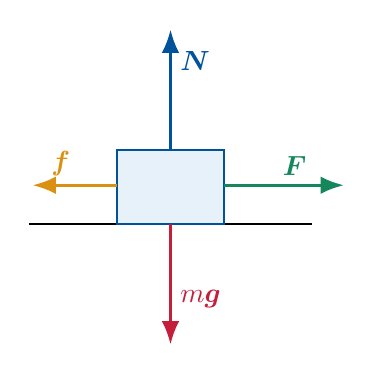
\begin{tikzpicture}[scale=0.9]
  \draw[thick] (-2,-0.7)--(2,-0.7);
  \fill[SoftBlue,draw=JapanBlue,thick] (-0.75,-0.7) rectangle (0.75,0.35);
  \forcearrow{0}{0.35}{0}{1.7}{JapanBlue}
  \forcearrow{0}{-0.7}{0}{-1.7}{ChinaRed}
  \forcearrow{0.75}{-0.15}{1.7}{0}{ForceGreen}
  \forcearrow{-0.75}{-0.15}{-1.2}{0}{ForceGold}
  \node[JapanBlue,right] at (0,1.6) {$\bm N$};
  \node[ChinaRed,right] at (0,-1.75) {$m\bm g$};
  \node[ForceGreen,above] at (1.75,-0.15) {$\bm F$};
  \node[ForceGold,above] at (-1.55,-0.15) {$\bm f$};
\end{tikzpicture}
\column{0.49\textwidth}
\begin{block}{四本の矢印を言葉にする}
\begin{itemize}
  \item 地球が物体を下向きに引く：重力
  \item 机が物体を上向きに押す：垂直抗力
  \item 人／绳が右向きに引く：外力
  \item 接触面が相对滑动を妨げる：摩擦力
\end{itemize}
\end{block}
\begin{alertblock}{判断原则}
每一支力的箭头都应能回答：\key{谁对谁施力？}
\end{alertblock}
\end{columns}
\end{frame}

\section{七つの重要な力}

\begin{frame}{1　重力（じゅうりょく）}
\begin{columns}[c]
\column{0.54\textwidth}
\begin{block}{重力 \en{weight / gravitational force near Earth}}
地球が物体を引く力：
\[
  \bm W=m\bm g,\qquad W=mg
\]
方向は鉛直下向き。EJU 中常用
\[
g=9.8\ \mathrm{m/s^2}\quad\text{或}\quad 10\ \mathrm{m/s^2}.
\]
\end{block}
\begin{alertblock}{質量との区別}
\jp{質量} $m$ 的单位是 kg，不随地点变化；\jp{重さ} $W$ 的单位是 N，会随 $g$ 改变。
\end{alertblock}
\column{0.4\textwidth}
\centering
\begin{tikzpicture}
  \shade[ball color=SoftBlue] (0,0) circle (0.8);
  \node at (0,0) {$m$};
  \forcearrow{0}{-0.8}{0}{-2.2}{ChinaRed}
  \node[ChinaRed,right] at (0,-2) {$\bm W=m\bm g$};
  \draw[GraphGray,dashed] (-1.4,-3.1)--(1.4,-3.1);
  \node[GraphGray] at (0,-3.45) {地球中心方向};
\end{tikzpicture}
\end{columns}
\end{frame}

\begin{frame}{例題 1｜重力：問題}
\vfill
\qcard{質量 $2.0\ \mathrm{kg}$ の物体が地球表面にある。$g=9.8\ \mathrm{m/s^2}$ として、重力の大きさと向きを求めよ。さらに月面で $g_{\rm moon}=1.6\ \mathrm{m/s^2}$ のときの重さも求めよ。}
\vfill
\end{frame}

\begin{frame}{例題 1｜重力：解答}
\acard{
地球上：
\[
W=mg=2.0\times9.8=\boxed{19.6\ \mathrm N}
\]
方向は\jp{鉛直下向き}。月面：
\[
W_{\rm moon}=2.0\times1.6=\boxed{3.2\ \mathrm N}.
\]
质量仍然是 $2.0\ \mathrm{kg}$，改变的是重力。}
\begin{alertblock}{检查}
答案若写成 $19.6\ \mathrm{kg}$，说明把质量单位和力的单位混淆了。
\end{alertblock}
\end{frame}

\begin{frame}{2　垂直抗力（すいちょくこうりょく）}
\begin{columns}[c]
\column{0.53\textwidth}
\begin{block}{垂直抗力 \en{normal force}}
接触面が物体を\key{面に垂直な方向}へ押す力，记作 $\bm N$。
\[
N\neq mg\quad\text{一般には}
\]
只有在特定平衡情形下两者数值才相等。
\end{block}
\begin{itemize}
  \item 水平面：方向竖直
  \item 斜面：方向垂直斜面
  \item 接触消失：$N=0$
\end{itemize}
\column{0.42\textwidth}
\centering
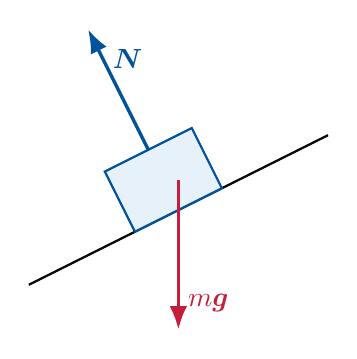
\begin{tikzpicture}[scale=0.95]
  \draw[thick] (-2,-1)--(2,1);
  \begin{scope}[rotate=26.565]
    \fill[SoftBlue,draw=JapanBlue,thick] (-0.65,0) rectangle (0.65,0.9);
    \forcearrow{0}{0.9}{0}{1.8}{JapanBlue}
    \node[JapanBlue,right] at (0,2.25) {$\bm N$};
  \end{scope}
  \forcearrow{0}{0.4}{0}{-2}{ChinaRed}
  \node[ChinaRed,right] at (0,-1.25) {$m\bm g$};
\end{tikzpicture}
\end{columns}
\end{frame}

\begin{frame}{例題 2｜垂直抗力：問題}
\vfill
\qcard{質量 $5.0\ \mathrm{kg}$ の箱が水平な床の上で静止している。人が箱を鉛直上向きに $15\ \mathrm N$ で引いている。床から受ける垂直抗力 $N$ を求めよ。$g=9.8\ \mathrm{m/s^2}$ とする。}
\vfill
\end{frame}

\begin{frame}{例題 2｜垂直抗力：解答}
\begin{columns}[c]
\column{0.44\textwidth}
\centering
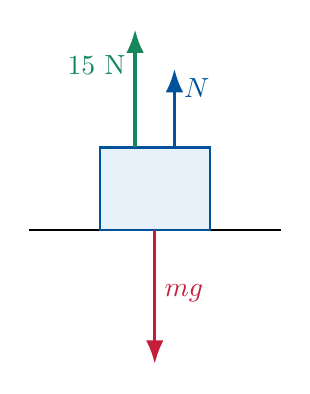
\begin{tikzpicture}
  \draw[thick] (-1.6,-0.8)--(1.6,-0.8);
  \fill[SoftBlue,draw=JapanBlue,thick] (-0.7,-0.8) rectangle (0.7,0.25);
  \forcearrow{-0.25}{0.25}{0}{1.5}{ForceGreen}
  \forcearrow{0.25}{0.25}{0}{1}{JapanBlue}
  \forcearrow{0}{-0.8}{0}{-1.7}{ChinaRed}
  \node[ForceGreen,left] at (-0.25,1.3) {$15$ N};
  \node[JapanBlue,right] at (0.25,1) {$N$};
  \node[ChinaRed,right] at (0,-1.6) {$mg$};
\end{tikzpicture}
\column{0.51\textwidth}
\acard{
鉛直方向のつり合い：
\[
N+15-mg=0
\]
\[
N=5.0\times9.8-15=\boxed{34\ \mathrm N}.
\]
向上的拉力承担了一部分重量，因此 $N<mg$。}
\end{columns}
\end{frame}

\begin{frame}{3　張力（ちょうりょく）}
\begin{columns}[c]
\column{0.54\textwidth}
\begin{block}{張力 \en{tension}}
張った糸・ロープが物体を\key{糸に沿って引く}力。
\begin{itemize}
  \item 绳只能拉，不能推
  \item 力的方向离开物体、沿绳指向外
  \item 理想轻绳＋光滑滑轮时，同一根绳张力相同
\end{itemize}
\end{block}
\begin{alertblock}{注意}
有质量的绳、粗糙或有转动惯量的滑轮，会使两侧张力不再相同。
\end{alertblock}
\column{0.4\textwidth}
\centering
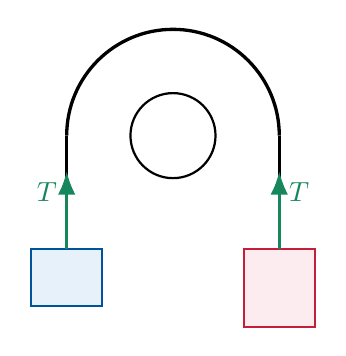
\begin{tikzpicture}[scale=0.9]
  \draw[very thick] (-1.5,1.8)--(-1.5,0.2);
  \draw[very thick] (1.5,1.8)--(1.5,0.2);
  \draw[very thick] (-1.5,1.8) arc[start angle=180,end angle=0,radius=1.5];
  \draw[thick] (0,1.8) circle (0.6);
  \fill[SoftBlue,draw=JapanBlue,thick] (-2,-0.6) rectangle (-1,0.2);
  \fill[SoftRed,draw=ChinaRed,thick] (1,-0.9) rectangle (2,0.2);
  \forcearrow{-1.5}{0.2}{0}{1.1}{ForceGreen}
  \forcearrow{1.5}{0.2}{0}{1.1}{ForceGreen}
  \node[ForceGreen,left] at (-1.5,1) {$T$};
  \node[ForceGreen,right] at (1.5,1) {$T$};
\end{tikzpicture}
\end{columns}
\end{frame}

\begin{frame}{例題 3｜張力：問題}
\vfill
\qcard{質量 $2.0\ \mathrm{kg}$ の物体を軽い糸で鉛直上向きに引くと、物体は上向きに $3.0\ \mathrm{m/s^2}$ で加速した。糸の張力 $T$ を求めよ。$g=9.8\ \mathrm{m/s^2}$。}
\vfill
\end{frame}

\begin{frame}{例題 3｜張力：解答}
\acard{
上向きを正にすると、
\[
T-mg=ma
\]
\[
T=m(g+a)=2.0(9.8+3.0)=\boxed{25.6\ \mathrm N}.
\]
加速度が上向きなので $T>mg$。若物体向上运动但正在减速，加速度实际上向下，不能只看速度方向。}
\begin{alertblock}{方向先行}
正方向を決めてから符号を代入する。公式を記憶するより自由体図が安全。
\end{alertblock}
\end{frame}

\begin{frame}{4　弾性力（だんせいりょく）}
\begin{columns}[c]
\column{0.55\textwidth}
\begin{block}{フックの法則 \en{Hooke's law}}
ばねの自然長からの変位を $x$ とすると：
\[
\bm F=-k\bm x,\qquad |F|=k|x|
\]
$k$：ばね定数 $[\mathrm{N/m}]$。负号表示弹力总是指向平衡位置。
\end{block}
\begin{itemize}
  \item 拉伸：弹簧向回拉
  \item 压缩：弹簧向外推
  \item 在弹性限度内才近似满足胡克定律
\end{itemize}
\column{0.39\textwidth}
\centering
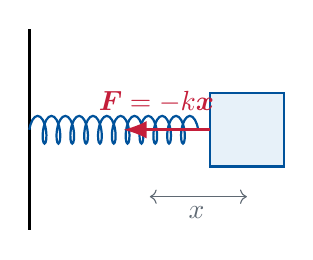
\begin{tikzpicture}[scale=0.85]
  \draw[very thick] (-2,1.5)--(-2,-1.5);
  \draw[decorate,decoration={coil,aspect=0.35,segment length=5pt,amplitude=5pt},thick,JapanBlue] (-2,0)--(0.7,0);
  \fill[SoftBlue,draw=JapanBlue,thick] (0.7,-0.55) rectangle (1.8,0.55);
  \forcearrow{0.7}{0}{-1.3}{0}{ChinaRed}
  \node[ChinaRed,above] at (-0.1,0.1) {$\bm F=-k\bm x$};
  \draw[<->,GraphGray] (-0.2,-1)--(1.25,-1);
  \node[GraphGray,below] at (0.5,-1) {$x$};
\end{tikzpicture}
\end{columns}
\end{frame}

\begin{frame}{例題 4｜弾性力：問題}
\vfill
\qcard{ばね定数 $k=200\ \mathrm{N/m}$ の軽いばねを自然長から $3.0\ \mathrm{cm}$ 伸ばした。ばねが物体に及ぼす弾性力の大きさを求めよ。変位を右向き正としたとき、力の符号も答えよ。}
\vfill
\end{frame}

\begin{frame}{例題 4｜弾性力：解答}
\acard{
まず $3.0\ \mathrm{cm}=0.030\ \mathrm m$ に直す。
\[
|F|=kx=200\times0.030=\boxed{6.0\ \mathrm N}
\]
右へ伸ばしたなら $x=+0.030\ \mathrm m$：
\[
F=-kx=\boxed{-6.0\ \mathrm N}.
\]
负号表示弹力向左，即恢复原长的方向。}
\begin{alertblock}{单位检查}
厘米不换成米会得到错误的 $600\ \mathrm N$。
\end{alertblock}
\end{frame}

\begin{frame}{5　摩擦力（まさつりょく）}
\begin{columns}[T]
\column{0.49\textwidth}
\begin{block}{静止摩擦力 \en{static friction}}
没有相对滑动时：
\[
0\le f_s\le \mu_s N
\]
它会“按需要”改变，并非总等于最大值。
\end{block}
\column{0.49\textwidth}
\begin{alertblock}{動摩擦力 \en{kinetic friction}}
已经滑动时：
\[
f_k=\mu_k N
\]
方向与接触面的\key{相对滑动方向}相反。
\end{alertblock}
\end{columns}
\vfill
\begin{center}
\begin{tikzpicture}[x=1cm,y=0.65cm]
  \draw[-{Latex}] (0,0)--(7.2,0) node[right] {外力 $F$};
  \draw[-{Latex}] (0,0)--(0,3.2) node[above] {摩擦力 $f$};
  \draw[very thick,JapanBlue] (0,0)--(3.5,2.4);
  \draw[dashed,GraphGray] (3.5,0)--(3.5,2.4);
  \draw[very thick,ChinaRed] (3.5,1.65)--(6.8,1.65);
  \node[JapanBlue,above left] at (3.5,2.4) {$f_{s,\max}=\mu_sN$};
  \node[ChinaRed,below] at (5.2,1.65) {$f_k=\mu_kN$};
  \node[GraphGray,below] at (3.5,0) {滑り始め};
\end{tikzpicture}
\end{center}
\end{frame}

\begin{frame}{摩擦力の方向を決める}
\begin{block}{判断顺序}
\begin{enumerate}
  \item 先假设没有摩擦，判断物体相对接触面的滑动趋势。
  \item 摩擦力与这个趋势相反。
  \item 用平衡或运动方程算出“所需静摩擦力”。
  \item 检查是否满足 $|f_s|\le\mu_sN$；超出则开始滑动，改用 $f_k=\mu_kN$。
\end{enumerate}
\end{block}
\begin{alertblock}{斜面上的典型情况}
物体有沿斜面下滑趋势时，静摩擦力沿斜面向上；但若外力强到使物体有上滑趋势，摩擦方向会反过来。
\end{alertblock}
\end{frame}

\begin{frame}{例題 5｜静止摩擦：問題}
\vfill
\qcard{質量 $4.0\ \mathrm{kg}$ の箱を水平面上で水平方向に $12\ \mathrm N$ で引く。静止摩擦係数は $\mu_s=0.40$ である。箱は動くか。動かない場合、摩擦力の大きさを求めよ。$g=9.8\ \mathrm{m/s^2}$。}
\vfill
\end{frame}

\begin{frame}{例題 5｜静止摩擦：解答}
\acard{
水平面なので $N=mg=39.2\ \mathrm N$。
\[
f_{s,\max}=\mu_sN=0.40\times39.2=15.68\ \mathrm N
\]
外力 $12\ \mathrm N<15.68\ \mathrm N$，箱は\key{動かない}。
平衡所需摩擦力就是
\[
\boxed{f_s=12\ \mathrm N}
\]
方向与拉力相反。}
\begin{alertblock}{关键}
不能一看到 $\mu_s$ 就写 $f_s=\mu_sN$；那只是最大值。
\end{alertblock}
\end{frame}

\begin{frame}{例題 6｜動摩擦：問題}
\vfill
\qcard{同じ $4.0\ \mathrm{kg}$ の箱を今度は $20\ \mathrm N$ で引く。箱が動き始めた後の動摩擦係数を $\mu_k=0.25$ とする。箱の加速度を求めよ。$g=9.8\ \mathrm{m/s^2}$。}
\vfill
\end{frame}

\begin{frame}{例題 6｜動摩擦：解答}
\acard{
\[
N=mg=39.2\ \mathrm N,\qquad
f_k=\mu_kN=0.25\times39.2=9.8\ \mathrm N
\]
水平方向：
\[
20-9.8=4.0a
\]
\[
a=\boxed{2.55\ \mathrm{m/s^2}}.
\]
动起来后用动摩擦系数，不能继续使用 $\mu_s$。}
\end{frame}

\begin{frame}{6　浮力（ふりょく）}
\begin{columns}[c]
\column{0.55\textwidth}
\begin{block}{アルキメデスの原理 \en{Archimedes' principle}}
流体から受ける浮力等于被排开流体的重量：
\[
F_B=\rho_{\rm fluid}gV_{\rm displaced}
\]
方向通常竖直向上。
\end{block}
\begin{itemize}
  \item 完全浸没：$V_{\rm displaced}=V_{\rm object}$
  \item 漂浮平衡：$F_B=mg$
  \item 看似重量：$W_{\rm app}=mg-F_B$
\end{itemize}
\column{0.4\textwidth}
\centering
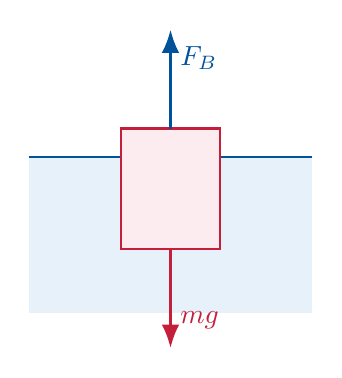
\begin{tikzpicture}[scale=0.9]
  \fill[SoftBlue] (-2,-1.8) rectangle (2,0.4);
  \draw[JapanBlue,thick] (-2,0.4)--(2,0.4);
  \fill[SoftRed,draw=ChinaRed,thick] (-0.7,-0.9) rectangle (0.7,0.8);
  \forcearrow{0}{0.8}{0}{1.4}{JapanBlue}
  \forcearrow{0}{-0.9}{0}{-1.4}{ChinaRed}
  \node[JapanBlue,right] at (0,1.8) {$F_B$};
  \node[ChinaRed,right] at (0,-1.9) {$mg$};
\end{tikzpicture}
\end{columns}
\end{frame}

\begin{frame}{例題 7｜浮力：問題}
\vfill
\qcard{体積 $2.0\times10^{-3}\ \mathrm{m^3}$ の物体を水中に完全に沈めた。水の密度を $1.0\times10^3\ \mathrm{kg/m^3}$ とする。浮力を求めよ。また物体の質量が $3.0\ \mathrm{kg}$ のとき、糸で静止させるための下向き／上向きの力を判断せよ。}
\vfill
\end{frame}

\begin{frame}{例題 7｜浮力：解答}
\acard{
\[
F_B=\rho gV=(1.0\times10^3)(9.8)(2.0\times10^{-3})=\boxed{19.6\ \mathrm N}
\]
重力は
\[
mg=3.0\times9.8=29.4\ \mathrm N.
\]
重力の方が $9.8\ \mathrm N$ 大きいので，静止させるには糸が\key{上向き}に
\[
\boxed{T=29.4-19.6=9.8\ \mathrm N}
\]
で引く。}
\end{frame}

\begin{frame}{7　万有引力（ばんゆういんりょく）}
\begin{columns}[c]
\column{0.57\textwidth}
\begin{block}{ニュートンの万有引力 \en{universal gravitation}}
二つの質点 $M,m$ 之间：
\[
F=G\frac{Mm}{r^2}
\]
方向は二物体を結ぶ直線上、互いに引き合う。
\[
G=6.67\times10^{-11}\ \mathrm{N\,m^2/kg^2}
\]
地表附近 $g=GM/R^2$，所以重力 $mg$ 是万有引力的近地面形式。
\end{block}
\column{0.37\textwidth}
\centering
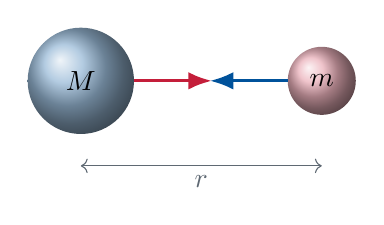
\begin{tikzpicture}[scale=0.9]
  \shade[ball color=JapanBlue!40] (-1.6,0) circle (0.75);
  \shade[ball color=ChinaRed!35] (1.8,0) circle (0.48);
  \node at (-1.6,0) {$M$};
  \node at (1.8,0) {$m$};
  \forcearrow{-0.85}{0}{1.1}{0}{ChinaRed}
  \forcearrow{1.32}{0}{-1.1}{0}{JapanBlue}
  \draw[<->,GraphGray] (-1.6,-1.2)--(1.8,-1.2);
  \node[GraphGray,below] at (0.1,-1.2) {$r$};
\end{tikzpicture}
\end{columns}
\end{frame}

\begin{frame}{例題 8｜万有引力：問題}
\vfill
\qcard{地球を半径 $R$、質量 $M$ の球とする。地表から高さ $h=R$ の位置（地球中心から $2R$）での重力加速度 $g'$ は、地表の $g$ の何倍か。物体の質量には依存するか。}
\vfill
\end{frame}

\begin{frame}{例題 8｜万有引力：解答}
\acard{
\[
g=\frac{GM}{R^2},\qquad
g'=\frac{GM}{(2R)^2}=\frac14\frac{GM}{R^2}
\]
したがって
\[
\boxed{g'=\frac14g}.
\]
$g'$ 不依赖被考察物体的质量；物体受到的引力 $F=mg'$ 才与自身质量成正比。}
\begin{alertblock}{反比例平方}
距离变为 $2$ 倍，力与重力加速度都变为 $1/2^2=1/4$。
\end{alertblock}
\end{frame}

\begin{frame}{例題 9｜七つの力を識別：問題}
\begin{columns}[c]
\column{0.44\textwidth}
\centering
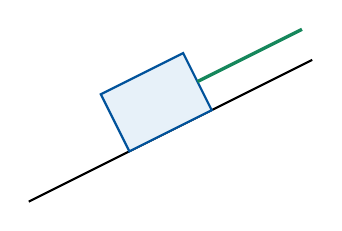
\begin{tikzpicture}[scale=0.9]
  \draw[thick] (-2,-1)--(2,1);
  \begin{scope}[rotate=26.565]
    \fill[SoftBlue,draw=JapanBlue,thick] (-0.65,0) rectangle (0.65,0.9);
    \draw[very thick,ForceGreen] (0.65,0.45)--(2.3,0.45);
  \end{scope}
\end{tikzpicture}
\column{0.52\textwidth}
\qcard{粗い斜面上の箱を、斜面に平行な糸で上向きに引いて静止させている。箱に作用する力をすべて挙げ、それぞれの方向を答えよ。摩擦力の向きは何によって決まるか。}
\end{columns}
\end{frame}

\begin{frame}{例題 9｜七つの力を識別：解答}
\begin{columns}[c]
\column{0.43\textwidth}
\centering
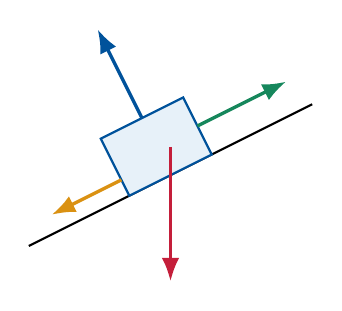
\begin{tikzpicture}[scale=0.9]
  \draw[thick] (-2,-1)--(2,1);
  \begin{scope}[rotate=26.565]
    \fill[SoftBlue,draw=JapanBlue,thick] (-0.65,0) rectangle (0.65,0.9);
    \forcearrow{0.65}{0.45}{1.4}{0}{ForceGreen}
    \forcearrow{0}{0.9}{0}{1.4}{JapanBlue}
    \forcearrow{-0.65}{0.25}{-1.1}{0}{ForceGold}
  \end{scope}
  \forcearrow{0}{0.4}{0}{-1.9}{ChinaRed}
\end{tikzpicture}
\column{0.52\textwidth}
\acard{
\begin{itemize}
  \item 重力 $mg$：鉛直下向き
  \item 垂直抗力 $N$：斜面に垂直
  \item 張力 $T$：糸に沿って斜面上向き
  \item 静止摩擦力 $f_s$：相对滑动趋势的反方向
\end{itemize}
若没有摩擦时箱有下滑趋势，摩擦向上；若拉力过大导致上滑趋势，摩擦向下。}
\end{columns}
\end{frame}

\begin{frame}{向心力は「第八の力」ではない}
\begin{block}{向心力 \en{centripetal force}}
円運動で中心向きの\key{合力}を呼ぶ名前：
\[
\sum F_{\rm inward}=m\frac{v^2}{r}
\]
它可能由张力、摩擦力、重力、垂直抗力等实际力提供。
\end{block}
\begin{columns}[c]
\column{0.44\textwidth}
\centering
\begin{tikzpicture}
  \draw[GraphGray,dashed] (0,0) circle (1.5);
  \fill[ChinaRed] (1.5,0) circle (0.12);
  \forcearrow{1.5}{0}{-1.4}{0}{JapanBlue}
  \node[JapanBlue,above] at (0.75,0) {$\sum\bm F$};
  \node at (0,-0.25) {中心};
\end{tikzpicture}
\column{0.51\textwidth}
\begin{alertblock}{语言陷阱}
“向心力”描述合力的功能和方向，不应在已经画出张力、重力等之后再额外多画一支向心力。
\end{alertblock}
\end{columns}
\end{frame}

\section{力のつり合い}

\begin{frame}{力のつり合い（ちからのつりあい）}
\begin{block}{平衡条件 \en{equilibrium}}
物体静止或做匀速直线运动时，加速度为零：
\[
\boxed{\sum\bm F=\bm0}
\]
二维问题必须同时满足：
\[
\boxed{\sum F_x=0},\qquad \boxed{\sum F_y=0}.
\]
\end{block}
\begin{alertblock}{平衡不等于没有力}
平衡是\key{合力为零}。物体可以同时受到多支非零的力；也可以正在以恒定速度运动。
\end{alertblock}
\end{frame}

\begin{frame}{力の分解と合成}
\begin{columns}[c]
\column{0.49\textwidth}
\begin{block}{成分分解}
若力 $F$ 与 $x$ 轴夹角为 $\theta$：
\[
F_x=F\cos\theta,\qquad F_y=F\sin\theta.
\]
斜面题常取：
\[
mg_{\parallel}=mg\sin\theta,
\quad mg_{\perp}=mg\cos\theta.
\]
\end{block}
\column{0.46\textwidth}
\centering
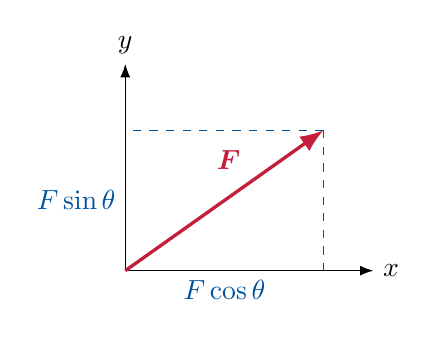
\begin{tikzpicture}[scale=1.05]
  \draw[-{Latex}] (0,0)--(3,0) node[right] {$x$};
  \draw[-{Latex}] (0,0)--(0,2.5) node[above] {$y$};
  \forcearrow{0}{0}{2.4}{1.7}{ChinaRed}
  \draw[dashed,JapanBlue] (2.4,1.7)--(2.4,0);
  \draw[dashed,JapanBlue] (2.4,1.7)--(0,1.7);
  \node[ChinaRed,above] at (1.25,1.1) {$\bm F$};
  \node[JapanBlue,below] at (1.2,0) {$F\cos\theta$};
  \node[JapanBlue,left] at (0,0.85) {$F\sin\theta$};
\end{tikzpicture}
\end{columns}
\end{frame}

\begin{frame}{平衡問題の標準手順}
\small
\stepbox{1　対象}{どの物体の平衡を調べるかを一つに絞る。}
\vspace{0.4em}
\stepbox{2　自由体図}{七つの力から、実際に作用する力だけを描く。}
\vspace{0.4em}
\stepbox{3　座標軸}{未知数が少なくなるように選ぶ。斜面軸、绳方向等。}
\vspace{0.4em}
\stepbox{4　成分式}{$\sum F_x=0,\ \sum F_y=0$。必要なら静摩擦上限も检查。}
\vspace{0.4em}
\stepbox{5　検算}{单位、正负号、极限情况、结果是否符合直觉。}
\end{frame}

\begin{frame}{例題 10｜二本の糸：問題}
\vfill
\qcard{質量 $10\ \mathrm{kg}$ の物体を二本の糸で静止させる。一方の糸は水平、他方の糸は水平となす角 $30^\circ$ で斜め上向きである。二本の糸の張力を求めよ。$g=9.8\ \mathrm{m/s^2}$。}
\vfill
\end{frame}

\begin{frame}{例題 10｜二本の糸：解答}
\begin{columns}[c]
\column{0.43\textwidth}
\centering
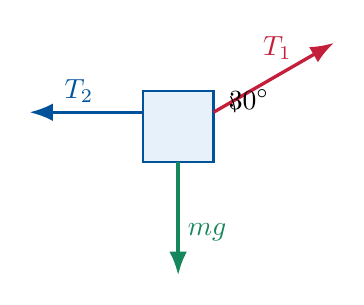
\begin{tikzpicture}[scale=0.9]
  \fill[SoftBlue,draw=JapanBlue,thick] (-0.5,-0.5) rectangle (0.5,0.5);
  \forcearrow{0.5}{0.2}{1.7}{0.98}{ChinaRed}
  \forcearrow{-0.5}{0.2}{-1.6}{0}{JapanBlue}
  \forcearrow{0}{-0.5}{0}{-1.6}{ForceGreen}
  \node[ChinaRed,above] at (1.4,0.8) {$T_1$};
  \node[JapanBlue,above] at (-1.4,0.2) {$T_2$};
  \node[ForceGreen,right] at (0,-1.5) {$mg$};
  \draw (0.8,0.2) arc[start angle=0,end angle=30,radius=0.45];
  \node at (1,0.38) {$30^\circ$};
\end{tikzpicture}
\column{0.52\textwidth}
\acard{
鉛直方向：$T_1\sin30^\circ=mg$，故
\[
T_1=\frac{98}{0.5}=\boxed{196\ \mathrm N}.
\]
水平方向：
\[
T_2=T_1\cos30^\circ=\boxed{170\ \mathrm N}\ (\text{约}).
\]}
\end{columns}
\end{frame}

\begin{frame}{例題 11｜斜面上の静止：問題}
\vfill
\qcard{傾角 $30^\circ$ の滑らかな斜面上に質量 $2.0\ \mathrm{kg}$ の物体がある。斜面に平行な糸で静止させるとき、張力 $T$ と垂直抗力 $N$ を求めよ。$g=9.8\ \mathrm{m/s^2}$。}
\vfill
\end{frame}

\begin{frame}{例題 11｜斜面上の静止：解答}
\acard{
斜面に平行・垂直な軸を取る：
\[
T-mg\sin30^\circ=0
\quad\Rightarrow\quad
T=2.0\times9.8\times0.5=\boxed{9.8\ \mathrm N}.
\]
\[
N-mg\cos30^\circ=0
\quad\Rightarrow\quad
N=19.6\times0.866=\boxed{17.0\ \mathrm N}\ (\text{约}).
\]
垂直抗力不负责抵消沿斜面的重力分量。}
\end{frame}

\begin{frame}{例題 12｜対称な二本の糸：問題}
\vfill
\qcard{質量 $10\ \mathrm{kg}$ の看板を、左右対称な二本の糸でつり下げる。各糸が水平となす角は $45^\circ$ である。各糸の張力 $T$ を求めよ。$g=9.8\ \mathrm{m/s^2}$。}
\vfill
\end{frame}

\begin{frame}{例題 12｜対称な二本の糸：解答}
\begin{columns}[c]
\column{0.43\textwidth}
\centering
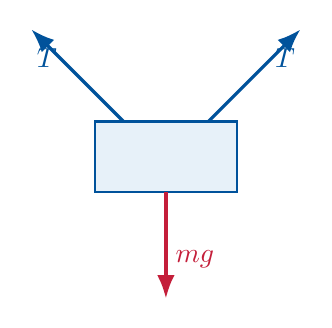
\begin{tikzpicture}[scale=0.9]
  \fill[SoftBlue,draw=JapanBlue,thick] (-1,-0.5) rectangle (1,0.5);
  \forcearrow{-0.6}{0.5}{-1.3}{1.3}{JapanBlue}
  \forcearrow{0.6}{0.5}{1.3}{1.3}{JapanBlue}
  \forcearrow{0}{-0.5}{0}{-1.5}{ChinaRed}
  \node[JapanBlue,left] at (-1.4,1.4) {$T$};
  \node[JapanBlue,right] at (1.4,1.4) {$T$};
  \node[ChinaRed,right] at (0,-1.45) {$mg$};
\end{tikzpicture}
\column{0.52\textwidth}
\acard{
水平分量彼此抵消。竖直方向：
\[
2T\sin45^\circ=mg=98\ \mathrm N
\]
\[
T=\frac{98}{2\times0.707}=\boxed{69.3\ \mathrm N}.
\]
绳越接近水平，所需张力越大。}
\end{columns}
\end{frame}

\begin{frame}{例題 13｜壁と静止摩擦：問題}
\vfill
\qcard{質量 $3.0\ \mathrm{kg}$ の物体を鉛直な壁に水平方向の力 $P$ で押しつけ、静止させる。物体と壁の静止摩擦係数は $\mu_s=0.40$ である。必要な $P$ の最小値を求めよ。$g=9.8\ \mathrm{m/s^2}$。}
\vfill
\end{frame}

\begin{frame}{例題 13｜壁と静止摩擦：解答}
\begin{columns}[c]
\column{0.4\textwidth}
\centering
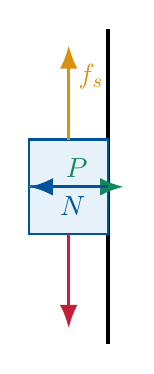
\begin{tikzpicture}
  \draw[very thick] (1,-2)--(1,2);
  \fill[SoftBlue,draw=JapanBlue,thick] (0, -0.6) rectangle (1,0.6);
  \forcearrow{0}{0}{1.2}{0}{ForceGreen}
  \forcearrow{1}{0}{-1}{0}{JapanBlue}
  \forcearrow{0.5}{0.6}{0}{1.2}{ForceGold}
  \forcearrow{0.5}{-0.6}{0}{-1.2}{ChinaRed}
  \node[ForceGreen,above] at (0.6,0) {$P$};
  \node[JapanBlue,below] at (0.55,0) {$N$};
  \node[ForceGold,right] at (0.5,1.4) {$f_s$};
\end{tikzpicture}
\column{0.55\textwidth}
\acard{
水平方向：$N=P$。竖直方向需要 $f_s=mg$。
刚好不下滑时：
\[
mg=f_{s,\max}=\mu_sN=\mu_sP
\]
\[
P_{\min}=\frac{3.0\times9.8}{0.40}=\boxed{73.5\ \mathrm N}.
\]}
\end{columns}
\end{frame}

\begin{frame}{例題 14｜浮いている物体：問題}
\vfill
\qcard{密度 $0.90\times10^3\ \mathrm{kg/m^3}$ の氷が、密度 $1.0\times10^3\ \mathrm{kg/m^3}$ の水に浮いて静止している。氷の全体積を $V$、水中部分を $V_s$ とするとき、$V_s/V$ を求めよ。}
\vfill
\end{frame}

\begin{frame}{例題 14｜浮いている物体：解答}
\acard{
浮いて静止：浮力＝重力。
\[
\rho_{\rm water}gV_s=\rho_{\rm ice}gV
\]
\[
\frac{V_s}{V}=\frac{\rho_{\rm ice}}{\rho_{\rm water}}
=\frac{0.90\times10^3}{1.0\times10^3}=\boxed{0.90}.
\]
因此约 $90\%$ 的体积在水下，$10\%$ 露出水面。结果与 $g$ 无关，因为两边约掉。}
\end{frame}

\begin{frame}{例題 15｜三力のつり合い：問題}
\vfill
\qcard{一点に三つの力が作用してつり合っている。既知の力 $\bm F$ の大きさは $10\ \mathrm N$、成分は左向き $8\ \mathrm N$、下向き $6\ \mathrm N$ である。他の二力はそれぞれ水平右向き $P$、鉛直上向き $Q$ である。$P,Q$ を求めよ。}
\vfill
\end{frame}

\begin{frame}{例題 15｜三力のつり合い：解答}
\begin{columns}[c]
\column{0.43\textwidth}
\centering
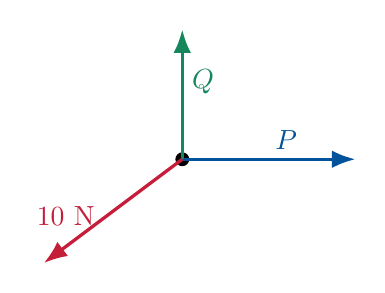
\begin{tikzpicture}[scale=1.1]
  \fill (0,0) circle (0.08);
  \forcearrow{0}{0}{2}{0}{JapanBlue}
  \forcearrow{0}{0}{0}{1.5}{ForceGreen}
  \forcearrow{0}{0}{-1.6}{-1.2}{ChinaRed}
  \node[JapanBlue,above] at (1.2,0) {$P$};
  \node[ForceGreen,right] at (0,0.9) {$Q$};
  \node[ChinaRed,left] at (-0.9,-0.65) {$10$ N};
\end{tikzpicture}
\column{0.52\textwidth}
\acard{
成分ごとに独立に平衡：
\[
\sum F_x=P-8=0\Rightarrow\boxed{P=8\ \mathrm N},
\]
\[
\sum F_y=Q-6=0\Rightarrow\boxed{Q=6\ \mathrm N}.
\]
$6$--$8$--$10$ 直角三角形也可用于检查。}
\end{columns}
\end{frame}

\section{総合練習}

\begin{frame}{総合例題 16｜粗い斜面：問題}
\small
\vfill
\qcard{質量 $5.0\ \mathrm{kg}$ の物体が傾角 $37^\circ$ の粗い斜面上にある。斜面に平行上向きの外力 $F$ を加えて静止させたい。静止摩擦係数は $\mu_s=0.50$。$\sin37^\circ=0.60,\ \cos37^\circ=0.80$ として、静止可能な $F$ の範囲を求めよ。$g=9.8\ \mathrm{m/s^2}$。}
\vfill
\end{frame}

\begin{frame}{総合例題 16｜粗い斜面：解答}
\small
\acard{
\[
mg\sin37^\circ=5.0\times9.8\times0.60=29.4\ \mathrm N,
\]
\[
N=mg\cos37^\circ=39.2\ \mathrm N,
\quad f_{s,\max}=0.50\times39.2=19.6\ \mathrm N.
\]
平衡所需摩擦力 $f_s=29.4-F$，条件
\[
|29.4-F|\le19.6.
\]
解得
\[
\boxed{9.8\ \mathrm N\le F\le49.0\ \mathrm N}.
\]
下限时有下滑趋势、摩擦向上；上限时有上滑趋势、摩擦向下。}
\end{frame}

\begin{frame}{総合例題 17｜滑車と摩擦：問題}
\vfill
\qcard{水平面上の $m_1=3.0\ \mathrm{kg}$ と、滑車を通して鉛直につるされた $m_2=2.0\ \mathrm{kg}$ が軽い糸で結ばれている。$m_1$ と面の静止摩擦係数は $0.30$、動摩擦係数は $0.20$。系は静止できるか。動くなら加速度を求めよ。}
\vfill
\end{frame}

\begin{frame}{総合例題 17｜滑車と摩擦：解答}
\small
\acard{
静止できるなら $T=m_2g=19.6\ \mathrm N$ が必要。一方，
\[
f_{s,\max}=\mu_sm_1g=0.30\times3.0\times9.8=8.82\ \mathrm N.
\]
不足なので静止できない。動摩擦は
\[
f_k=0.20\times3.0\times9.8=5.88\ \mathrm N.
\]
二物体を一つの系として：
\[
m_2g-f_k=(m_1+m_2)a
\]
\[
a=\frac{19.6-5.88}{5.0}=\boxed{2.74\ \mathrm{m/s^2}}.
\]}
\end{frame}

\begin{frame}{確認練習｜問題}
\small
\begin{enumerate}
  \item 質量 $6.0\ \mathrm{kg}$ の箱を水平面上で上向き $20\ \mathrm N$ に引く。静止時の $N$ は？
  \item $k=150\ \mathrm{N/m}$ のばねを $4.0\ \mathrm{cm}$ 圧縮したときの弾性力は？
  \item $\mu_s=0.50$、$N=40\ \mathrm N$。外力 $12\ \mathrm N$ で静止している物体の摩擦力は？
  \item 同じ二本の糸で荷物をつるすとき、糸を水平に近づけると張力はどうなる？
  \item 高さが地球半径の $2R$、すなわち中心から $3R$ の点で $g'$ は地表の何倍？
  \item 等速円運動中の「向心力」は、新しい種類の力か？
\end{enumerate}
\end{frame}

\begin{frame}{確認練習｜解答}
\small
\begin{enumerate}
  \item $N=mg-20=6.0\times9.8-20=\boxed{38.8\ \mathrm N}$。
  \item $F=kx=150\times0.040=\boxed{6.0\ \mathrm N}$，方向は自然長へ戻る向き。
  \item $f_s=\boxed{12\ \mathrm N}$。最大値 $20\ \mathrm N$ ではない。
  \item 鉛直分量を保つため、張力は\key{大きくなる}。
  \item $g'/g=R^2/(3R)^2=\boxed{1/9}$。
  \item 不是。中心方向的\key{合力}，由实际力提供。
\end{enumerate}
\end{frame}

\begin{frame}{まとめ：力を見抜くチェックリスト}
\begin{columns}[T]
\column{0.49\textwidth}
\begin{block}{接触しなくても働く}
\begin{itemize}
  \item 重力 $mg$
  \item 万有引力 $GMm/r^2$
\end{itemize}
\end{block}
\begin{block}{接触によって働く}
\begin{itemize}
  \item 垂直抗力
  \item 摩擦力
  \item 浮力（流体との接触）
\end{itemize}
\end{block}
\column{0.49\textwidth}
\begin{alertblock}{連結によって働く}
\begin{itemize}
  \item 張力
  \item 弾性力
\end{itemize}
\end{alertblock}
\begin{exampleblock}{解题核心}
\begin{enumerate}
  \item 谁对谁施力？
  \item 方向是什么？
  \item 是否平衡？
  \item 静摩擦是否超过上限？
\end{enumerate}
\end{exampleblock}
\end{columns}
\end{frame}

\begin{frame}{宿題}
\small
\begin{enumerate}
  \item 电梯内 $60\ \mathrm{kg}$ 的人以 $1.5\ \mathrm{m/s^2}$ 向上加速，求地板支持力。
  \item $25^\circ$ 光滑斜面上 $3.0\ \mathrm{kg}$ 物体由平行斜面的绳保持静止，求 $T,N$。
  \item 水平面上箱子 $mu_s=0.35,\mu_k=0.20$，逐渐增大外力，画摩擦力随外力变化的图。
  \item 两根对称绳与竖直方向各成 $60^\circ$，悬挂 $5.0\ \mathrm{kg}$ 物体，求张力。
  \item 密度 $0.75\times10^3\ \mathrm{kg/m^3}$ 的木块漂浮在水面，求浸没比例。
  \item 粗糙斜面综合题：自行改变例题16中的 $\mu_s$，说明允许外力范围如何变化。
\end{enumerate}
\vfill
\centering
\jp{先画自由体图，再列方程；图比公式更重要。}
\end{frame}

\end{document}
